La presente sección tiene como objetivo predecir la cantidad de muertes por cáncer de pulmón en México utilizando dos enfoques distintos: \textbf{Regresión Lineal} y una \textbf{Red Neuronal Recurrente (LSTM)}. A través de esta comparación, se busca evaluar la precisión de ambos modelos y determinar cuál ofrece mejores resultados para la proyección de datos futuros.

Las versiones de \textit{Python} fueron las siguientes:

\begin{itemize}
    \item TensorFlow versión: 2.10.0
    \item NumPy versión: 1.26.4
    \item Matplotlib versión: 3.7.1
    \item Sklearn versión: 1.3.2
    \item Python versión: 3.8.0
\end{itemize}

Para el análisis, se utilizó un conjunto de datos que contiene el registro anual de muertes por una gran cantidad de tipos de cáncer en todo el mundo desde 1990 hasta 2016. Este dataset fue obtenido de la plataforma Kaggle, específicamente del conjunto de datos:
\href{https://www.kaggle.com/datasets/antimoni/cancer-deaths-by-country-and-type-1990-2016}{\textit{"Cancer Deaths by Country and Type (1990-2016)"}}.


Dicho dataset recopila la cantidad de muertes por distintos tipos de cáncer en múltiples países. Sin embargo, dado que este estudio se enfoca exclusivamente en México, se realizó una preprocesamiento de los datos para filtrar únicamente la información relevante al país. Esta versión depurada del dataset nos permite analizar la cantidad de muertes causadas por algún tipo de cáncer que ha habido en el país de 1990 al 2016. 


\begin{table}[h!]
    \centering
    \begin{tabular}{|c|c|c|c|c|}
    \hline
    \textbf{Year} & \textbf{Liver cancer} & \textbf{Kidney cancer} & \textbf{Larynx cancer} & \textbf{...}\\ \hline
    1990 & 2995.515782 & 867.859970 & 765.007794 & ...\\ \hline
    1991 & 3072.586220 & 903.779729 & 776.570274 & ...\\ \hline
    1992 & 3194.398432 & 947.317928 & 796.109315 & ...\\ \hline
    1993 & 3318.471538 & 977.590436 & 809.788569 & ...\\ \hline
    1994 & 3431.584846 & 1018.196197 & 818.597311 & ...\\ \hline
    ... & ... & ... & ... & ...\\ \hline
    \end{tabular}
    \caption{Ejemplo del dataset Cancer deaths mexico}
    \label{table:cancer_cases}
\end{table}



Como punto de partida en el análisis exploratorio, se presenta un gráfico que muestra la evolución de las muertes por diferentes tipos de cáncer en México. Esto permite visualizar las diferencias en la mortalidad a lo largo del tiempo y comprender la relevancia del cáncer de pulmón en el contexto general.

\begin{figure}[h!] 
    \centering 
    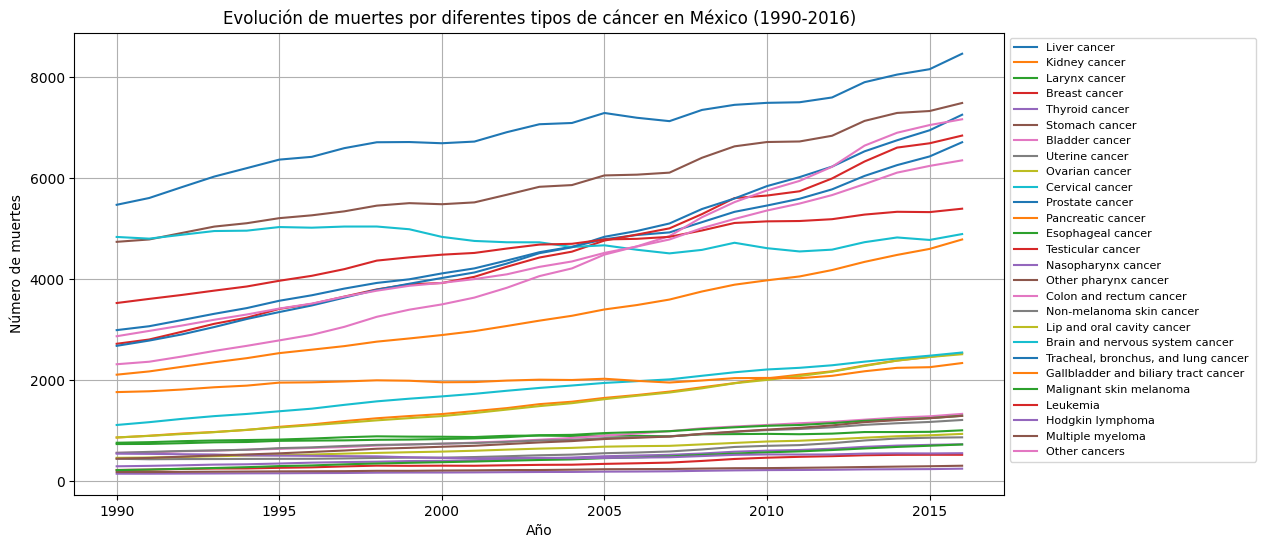
\includegraphics[width=1.0\textwidth]{Zdenko/Imágenes/canceres.png}
    \caption{Comparación de muertes entre diferentes tipos de cáncer en México} 
    \label{fig:comparacion_canceres} 
\end{figure}


Dado que el enfoque de este estudio es el cáncer de pulmón, se llevó a cabo una segunda fase de preprocesamiento para extraer exclusivamente los registros relacionados con esta enfermedad, modificando el dataset y dejando únicamente los anos y las cantidades de muertes. 

\begin{table}[h!]
    \centering
    \begin{tabular}{|c|c|}
    \hline
    \textbf{Year} & \textbf{Tracheal, bronchus, and lung cancer} \\ \hline
    1990 & 5477.606751 \\ \hline
    1991 & 5612.037783 \\ \hline
    1992 & 5826.280440 \\ \hline
    1993 & 6036.566757 \\ \hline
    1994 & 6203.391357 \\ \hline
    1995 & 6372.230116 \\ \hline
    1996 & 6427.327966 \\ \hline
    1997 & 6599.432588 \\ \hline
    ... & ... \\ \hline
    \end{tabular}
    \caption{Evolución de casos de cáncer traqueal, bronquial y pulmonar}
    \label{table:lung_cancer}
\end{table}


Este análisis exploratorio inicial permite observar de manera detallada la evolución de la mortalidad por cáncer de pulmón en México, identificando posibles tendencias y patrones de crecimiento. Al examinar la variación en el número de muertes anuales, se pueden detectar periodos de mayor incidencia, así como evaluar la estabilidad o fluctuaciones en la progresión de la enfermedad.

Estos hallazgos resultan fundamentales para comprender el comportamiento histórico de los datos y proporcionan una base sólida para la implementación de los modelos predictivos en las siguientes secciones. Con esta información, se busca desarrollar algoritmos capaces de estimar con mayor precisión la evolución futura de las muertes por cáncer de pulmón, permitiendo una comparación efectiva entre los enfoques de Regresion lineal y redes neuronales recurrentes (LSTM).

Para ilustrar la evolución de las muertes por cáncer de pulmón en México a lo largo del tiempo, se presenta el siguiente histograma:

\begin{figure}[h] \centering 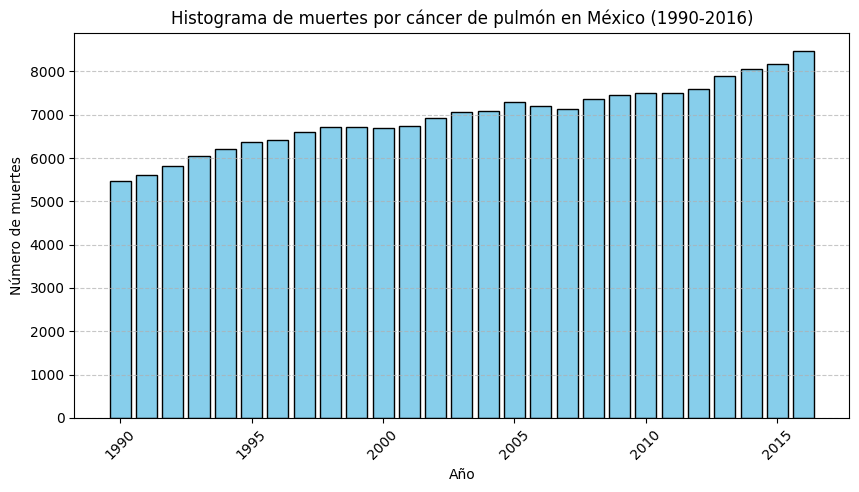
\includegraphics[width=1.0\textwidth]{Zdenko/Imágenes/histograma.png} \caption{Evolución de muertes por cáncer de pulmón en México} \label{fig:histograma_pulmon} \end{figure}

Se realizó el cálculo de la media móvil, generando el siguiente gráfico. Este método es clave para suavizar fluctuaciones y resaltar tendencias subyacentes en los datos. Al eliminar el ruido, facilita una interpretación más clara y apoya el desarrollo de estrategias predictivas más precisas.

\lstset{
    language=Python,
    basicstyle=\ttfamily\footnotesize,
    keywordstyle=\color{blue},
    commentstyle=\color{gray},
    stringstyle=\color{green!60!black},
    numberstyle=\tiny\color{gray},
    numbers=left,
    breaklines=true,
    frame=single,
    captionpos=b,
    tabsize=4,
    showspaces=false,
    showstringspaces=false,
    showtabs=false
}

El cálculo de la media móvil de 5 anos se realiza con el siguiente código Python:

\begin{lstlisting}
df_mexico_lung["Moving_Avg_5"] = df_mexico_lung["Tracheal, bronchus, and lung cancer"].rolling(window=5).mean()
\end{lstlisting}

Este código aplica una media móvil utilizando una ventana de 5 anos para los valores en la columna específica.

\begin{figure}[h] \centering 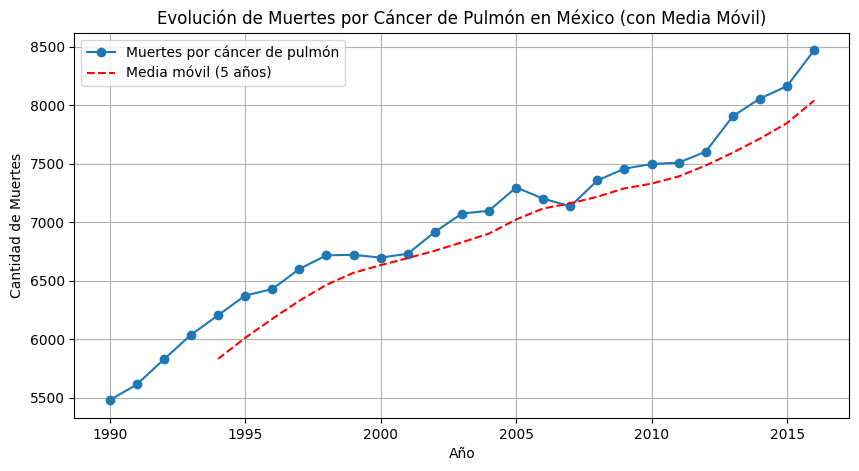
\includegraphics[width=1.0\textwidth]{Zdenko/Imágenes/media_movil.png} \caption{Media móvil en la evolución de muertes por cáncer de pulmón en México} \label{fig:media_movil} \end{figure}

Complementando el histograma y la media móvil, se realizaron los cálculos de la tasa de crecimiento anual:

\lstset{
    language=Python,
    basicstyle=\ttfamily\footnotesize,
    keywordstyle=\color{blue},
    commentstyle=\color{gray},
    stringstyle=\color{green!60!black},
    numberstyle=\tiny\color{gray},
    numbers=left,
    breaklines=true,
    frame=single,
    captionpos=b,
    tabsize=4,
    showspaces=false,
    showstringspaces=false,
    showtabs=false
}

\begin{lstlisting}
# Calcular la tasa de crecimiento anual
df['Tasa de Crecimiento (%)'] = df['Tracheal, bronchus, and lung cancer'].pct_change() * 100

# Calcular el Crecimiento Anual Compuesto (CAGR)
valor_inicial = df['Tracheal, bronchus, and lung cancer'].iloc[0]
valor_final = df['Tracheal, bronchus, and lung cancer'].iloc[-1]
anos = df['Year'].iloc[-1] - df['Year'].iloc[0]

CAGR = ((valor_final / valor_inicial) ** (1/anos) - 1) * 100

print(f"Tasa de Crecimiento Anual Compuesto (CAGR): {CAGR:.2f}%")
print(df[['Year', 'Tracheal, bronchus, and lung cancer', 'Tasa de Crecimiento (%)']])
\end{lstlisting}

Este código realiza cálculos clave para analizar la evolución de las tasas de crecimiento anual. 

EL cual, la Tasa de Crecimiento Anual Compuesto es del \textbf{1.69}%.
Tal Crecimiento Anual Compuesto se desglosa de la siguiente manera: 

\begin{table}[h!]
\centering
\begin{tabular}{|c|c|c|}
\hline
\textbf{Year} & \textbf{Tracheal, bronchus, and lung cancer} & \textbf{Tasa de Crecimiento (\%)} \\ \hline
1990 & 5477.606751 & NaN \\ \hline
1991 & 5612.037783 & 2.45 \\ \hline
1992 & 5826.280440 & 3.82 \\ \hline
1993 & 6036.566757 & 3.61 \\ \hline
1994 & 6203.391357 & 2.76 \\ \hline
1995 & 6372.230116 & 2.72 \\ \hline
1996 & 6427.327966 & 0.86 \\ \hline
1997 & 6599.432588 & 2.68 \\ \hline
1998 & 6716.166865 & 1.77 \\ \hline
1999 & 6720.453596 & 0.06 \\ \hline
2000 & 6696.652587 & -0.35 \\ \hline
2001 & 6729.512760 & 0.49 \\ \hline
2002 & 6915.995188 & 2.77 \\ \hline
2003 & 7072.815396 & 2.27 \\ \hline
2004 & 7097.696918 & 0.35 \\ \hline
2005 & 7295.835659 & 2.79 \\ \hline
2006 & 7201.171839 & -1.30 \\ \hline
2007 & 7134.160110 & -0.93 \\ \hline
2008 & 7356.270666 & 3.11 \\ \hline
2009 & 7457.153413 & 1.37 \\ \hline
2010 & 7496.590945 & 0.53 \\ \hline
2011 & 7508.335423 & 0.16 \\ \hline
2012 & 7603.165121 & 1.26 \\ \hline
2013 & 7905.750272 & 3.98 \\ \hline
2014 & 8056.332637 & 1.90 \\ \hline
2015 & 8162.953063 & 1.32 \\ \hline
2016 & 8469.498356 & 3.76 \\ \hline
\end{tabular}
\caption{Casos de cáncer traqueal, bronquial y pulmonar, y su tasa de crecimiento anual (1990-2016)}
\label{table:cancer_growth}
\end{table}

Teniendo presentes tales dimensiones de la enfermedad, daremos inicio al modelo de Regresion Lineal.
\newpage
\subsubsection{Modelo de Regresión Lineal}
Se implementó un modelo de \textbf{Regresión Lineal} para predecir las muertes futuras. Se ajustó una línea de tendencia sobre los datos de entrenamiento y se proyectaron valores hasta el año 2040.

\begin{lstlisting}[language=Python, caption=Código de Regresion Lineal]
import pandas as pd
import numpy as np
import matplotlib.pyplot as plt
from sklearn.linear_model import LinearRegression

Cargar datos

df = pd.read_csv("Muertes_Mexico.csv")
X = df[["Year"]].values
y = df["Tracheal, bronchus, and lung cancer "]

Entrenamiento del modelo

modelo = LinearRegression()
modelo.fit(X, y)

Prediccion para el 2040

anio_futuro = np.array([[2040]])
muertes_2040 = modelo.predict(anio_futuro)
print(f"Prediccion de muertes para el ano 2040: {muertes_2040[0]:.2f}")
\end{lstlisting}

\subsubsection{Red Neuronal Recurrente (LSTM)}

Se implementó una red neuronal recurrente del tipo LSTM para comparar la Predicción de los datos temporales. En contraste con el Modelo de Regresion Lineal, se normalizaron los datos antes del entrenamiento.

\lstset{
    language=Python,
    basicstyle=\ttfamily\footnotesize,
    keywordstyle=\color{blue},
    commentstyle=\color{gray},
    stringstyle=\color{green!60!black},
    numberstyle=\tiny\color{gray},
    numbers=left,
    breaklines=true,
    frame=single,
    captionpos=b,
    tabsize=4,
    showspaces=false,
    showstringspaces=false,
    showtabs=false
}

\begin{lstlisting}[language=Python, caption=Modelo LSTM]
from sklearn.preprocessing import MinMaxScaler
from tensorflow.keras.models import Sequential
from tensorflow.keras.layers import LSTM, Dense, Dropout
from tensorflow.keras.callbacks import EarlyStopping
from sklearn.metrics import mean_squared_error

X = df[["Year"]].values
y = df["Tracheal, bronchus, and lung cancer"].values

# Normalizar los datos
scaler_x = MinMaxScaler()
X_scaled = scaler_x.fit_transform(X)

scaler_y = MinMaxScaler()
y_scaled = scaler_y.fit_transform(y.reshape(-1, 1))

# Crear secuencias para la LSTM
def create_sequences(X_data, y_data, seq_length):
    sequences, labels = [], []
    for i in range(len(X_data) - seq_length):
        sequences.append(np.hstack((X_data[i:i + seq_length], y_data[i:i + seq_length])))
        labels.append(y_data[i + seq_length])
    return np.array(sequences), np.array(labels)

seq_length = 5  
X_seq, y_seq = create_sequences(X_scaled, y_scaled, seq_length)

# Division de datos en entrenamiento y prueba
split = int(0.8 * len(X_seq))
X_train, X_test = X_seq[:split], X_seq[split:]
y_train, y_test = y_seq[:split], y_seq[split:]

# Construccion del modelo LSTM optimizado
model = Sequential([
    LSTM(32, activation='tanh', return_sequences=True, input_shape=(seq_length, 2)),
    Dropout(0.2),
    LSTM(16, activation='tanh'),
    Dropout(0.2),
    Dense(10, activation='relu'),
    Dense(1)])

# Compilar el modelo
model.compile(optimizer='adam', loss='mse')

# Usar Early Stopping para evitar sobreentrenamiento
early_stop = EarlyStopping(monitor='val_loss', patience=10, restore_best_weights=True)

# Entrenar el modelo
model.fit(X_train, y_train, epochs=200, batch_size=16, validation_data=(X_test, y_test), callbacks=[early_stop])

# Hacer predicciones futuras hasta 2040
anos_futuros = np.arange(X.min(), 2041).reshape(-1, 1)
anos_futuros_scaled = scaler_x.transform(anos_futuros)

future_preds = []
input_seq = X_seq[-1].copy()

for _ in range(2040 - X.max()):
    pred = model.predict(input_seq.reshape(1, seq_length, 2))[0]
    future_preds.append(pred)
    input_seq = np.roll(input_seq, -1, axis=0)
    input_seq[-1] = np.hstack((anos_futuros_scaled[len(future_preds) - 1], pred))

# Desnormalizar predicciones
future_preds = scaler_y.inverse_transform(np.array(future_preds).reshape(-1, 1))

mse_regresion = mean_squared_error(y_test, y_pred)
mse_lstm = mean_squared_error(y_test, y_pred_lstm)

print(f"MSE Regresion Lineal: {mse_regresion}")
print(f"MSE LSTM: {mse_lstm}")
\end{lstlisting}
